\documentclass[12pt,a4paper]{article}
\usepackage[utf8]{inputenc}
\usepackage[czech]{babel}
\usepackage[T1]{fontenc}
\usepackage{graphicx}
\usepackage[left=2cm,right=2cm,top=2cm,bottom=2cm]{geometry}
\usepackage{mathtools}
%\usepackage{cancel}
\usepackage{newtxtext,newtxmath}
\author{Ondřej Ondryáš\\František Nečas\\David Chocholatý\\David Mihola\\Lukáš Foltyn}
\title{IDM – Domácí úloha}

\newcommand{\pageline}{\noindent\makebox[\linewidth]{\rule{\linewidth}{0.4pt}}\vspace{5pt}}
\setlength{\parskip}{0.75em}


\begin{document}
\maketitle

\setlength\abovedisplayshortskip{10pt}
\setlength\abovedisplayskip{10pt}
\setlength\belowdisplayshortskip{10pt}
\setlength\belowdisplayskip{10pt}

\section*{Příklad 1}

Dokažte, že pro každé přirozené číslo \(n \geq 2\) platí:
\[
	\frac{1}{2} \cdot \frac{3}{4} \cdot ... \cdot \frac{2n-1}{2n} < \frac{1}{\sqrt{2n + 1}}
\]
\pageline

V prvním kroku matematické indukce ukážeme, že nerovnost platí pro nejmenší možné přirozené číslo odpovídající zadání:
\begin{gather*}
	L(2) = \frac{1}{2} \cdot \frac{3}{4} = \frac{3}{8} = \frac{15}{40} \\
    P(2) = \frac{1}{\sqrt{5}} = \frac{\sqrt{5}}{5} = \frac{8\sqrt{5}}{40} \\
    \sqrt{5} > \sqrt{4} \Rightarrow \frac{8\sqrt{5}}{40} > \frac{8\sqrt{4}}{40} \iff \frac{8\sqrt{5}}{40} > \frac{16}{40} \Rightarrow \frac{8\sqrt{5}}{40} > \frac{15}{40} \\
	L(2) < P(2)
\end{gather*}

Jestliže pro každé $k \geq 2, k \in \mathbb{N}$ platí:
\[
    V(k): \frac{1}{2} \cdot \frac{3}{4} \cdot ... \cdot \frac{2k-1}{2k} < \frac{1}{\sqrt{2k + 1}},
\]
pak potřebujeme dokázat, že nerovnost platí i pro $n=k+1$, tedy že platí:
\[
    V(k+1): \frac{1}{2} \cdot \frac{3}{4} \cdot ... \cdot \frac{2k-1}{2k} \cdot \frac{2k+1}{2k+2} < \frac{1}{\sqrt{2k + 3}}.
\]

Dle indukčního předpokladu platí:
\[
    \frac{1}{2} \cdot \frac{3}{4} \cdot ... \cdot \frac{2k-1}{2k} \cdot \frac{2k+1}{2k+2} < \frac{1}{\sqrt{2k + 1}} \cdot \frac{2k+1}{2k + 2},
\]
stačí tedy ukázat, že platí:
\[
    \frac{1}{\sqrt{2k+1}} \cdot \frac{2k+1}{2k+2} < \frac{1}{\sqrt{2k+3}}.
\]
Nerovnici můžeme dále upravovat, protože $k \geq 2 \Rightarrow 2k + 2 > 0$:
\begin{gather*}
    \frac{\sqrt{2k+1}}{2k+2} < \frac{1}{\sqrt{2k+3}} \\
    \sqrt{2k+1} \cdot \sqrt{2k+3} < 2k+2, \\
    4k^2 + 8k + 3 < 4k^2 + 8k + 4, \\
    3 < 4.
\end{gather*}
Tím je dokázáno, že zadaná nerovnice platí i pro $n = k + 1$. $\blacksquare$

\newpage

\section*{Příklad 2}

Na množině přirozených čísel je dána relace následovně:
\begin{equation*}
    a \sim b \iff a \cdot b \text{ je druhou mocninou přirozeného čísla}.
\end{equation*}
Zjistěte, zda $\sim$ je ekvivalence nebo uspořádání (případně ani jedno) na množině $\mathbb{N}$.

\pageline

Relace ekvivalence je binární relace na množině, která je reflexivní, symetrická a tranzitivní.
\[
    \forall a \in \mathbb{N}: a \cdot a = a^2 \Rightarrow \forall a \in \mathbb{N}: a \sim a.
\]
Relace je reflexivní.

Protože násobení je komutativní operace, platí, že:
\[
    \text{Nechť } a \sim b \Rightarrow a \cdot b = n^2 \Rightarrow b \cdot a = n^2 \Rightarrow b \sim a.
\]
Relace je symetrická.
\begin{multline*}
\text{Nechť } a \sim b \land b \sim c \Rightarrow \exists n,m \in \mathbb{N}: a \cdot b = n^2 \land b \cdot c = m^2 \Rightarrow a \cdot b^2 \cdot c = n^2 \cdot m^2\\ \Rightarrow a \cdot c = \frac{n^2 \cdot m^2}{b^2} \Rightarrow a \cdot c = \left(\frac{n \cdot m}{b}\right)^2.
\end{multline*}
%Nyní musíme dokázat, že
%\[
%	a,b,c,n,m \in \mathbb{N} \land a \cdot b = n^2 \land b \cdot c = m^2 \Rightarrow %\frac{n\cdot m}{b} \in \mathbb{N} 
%\]
%Využijeme k tomu důkaz sporem:
%\begin{gather*}
%a
%\end{gather*}
Relace je tranzitivní.

Relace by byla uspořádáním, kdyby platilo, že je reflexivní, antisymetrická a tranzitivní. Reflexivitu a tranzitivitu jsme již dokázali.

Aby byla relace antisymetrická, muselo by platit:
\[
   \forall a,b \in \mathbb{N}: a \sim b \land b \sim a \Rightarrow a = b.
\]
To ovšem neplatí, neboť druhá mocnina přirozeného čísla může vzniknout vynásobením dvou různých čísel:
\[
   \text{Nechť } a = 1, b = 4 \Rightarrow a \neq b \land a \cdot b = b \cdot a = 1 \cdot 4 = 4 \cdot 1 = 2^2 \Rightarrow a \sim b \land b \sim a \land a \neq b.
\]

Relace je reflexivní, symetrická a tranzitivní, jedná se tak o relaci ekvivalence. Protože relace není antisymetrická, není uspořádáním.

\newpage

\section*{Příklad 3}
Najděte všechna $x \in \mathbb{R},$ pro která mají intervaly \(\left\langle 3, \frac{x^2-x}{2} \right\rangle, \left\langle x+2, \infty \right\rangle \) alespoň dva společné body.
\pageline

Pro řešení z definice intervalu vyplývá, že:
\begin{gather*}
\frac{x^2-x}{2}>3 \Rightarrow x^2-x-6>0 \Rightarrow (x-3)(x+2)>0 \\
x \in \left(-\infty , -2\right) \cup \left(3, \infty \right)
\end{gather*}

Aby měly tyto intervaly neprázdný průnik, musí platit:
\begin{align*}
\frac{x^2-x}{2}&>x+2 \\
x^2-x&>2x+4 \\
x^2-3x-4&>0 \\
(x+1)(x-4)&>0 \\
x \in \left(-\infty , 1\right) &\cup \left(4, \infty \right)
\end{align*}
Nerovnost je v tomto případě ostrá, protože intervaly mají mít dva společné body. Kdyby se horní mez prvního a spodní mez druhého intervalu rovnaly, intervaly by měly pouze jeden společný bod.

Intervaly tak mají dva společné body, pokud:
\[
x \in \left(-\infty , -2\right) \cup \left(3, \infty \right) \land x \in \left(-\infty , 1\right) \cup \left(4, \infty \right) \Rightarrow x \in \left(-\infty , -2\right) \cup \left(4, \infty \right).
\]

\newpage
\section*{Příklad 4}
Rozhodněte o pravdivosti následujícího výroku:
\textit{Nechť $T$ je tranzitivní relace na množině $M$, potom také relace $\overline{T}$ je
tranzitivní na množině M.}

\pageline

Nechť \(M=\{0,1,2,3\},\ T=\{(0,1), (1,2), (0,2)\}\). Potom \(\overline{T}\supseteq \{(0,3),(3,2)\}\), ale \((0,2)\notin \overline{T}\), protože \((0,2)\in T\). Výrok je nepravdivý.

\begin{figure}[h]
 \centering
 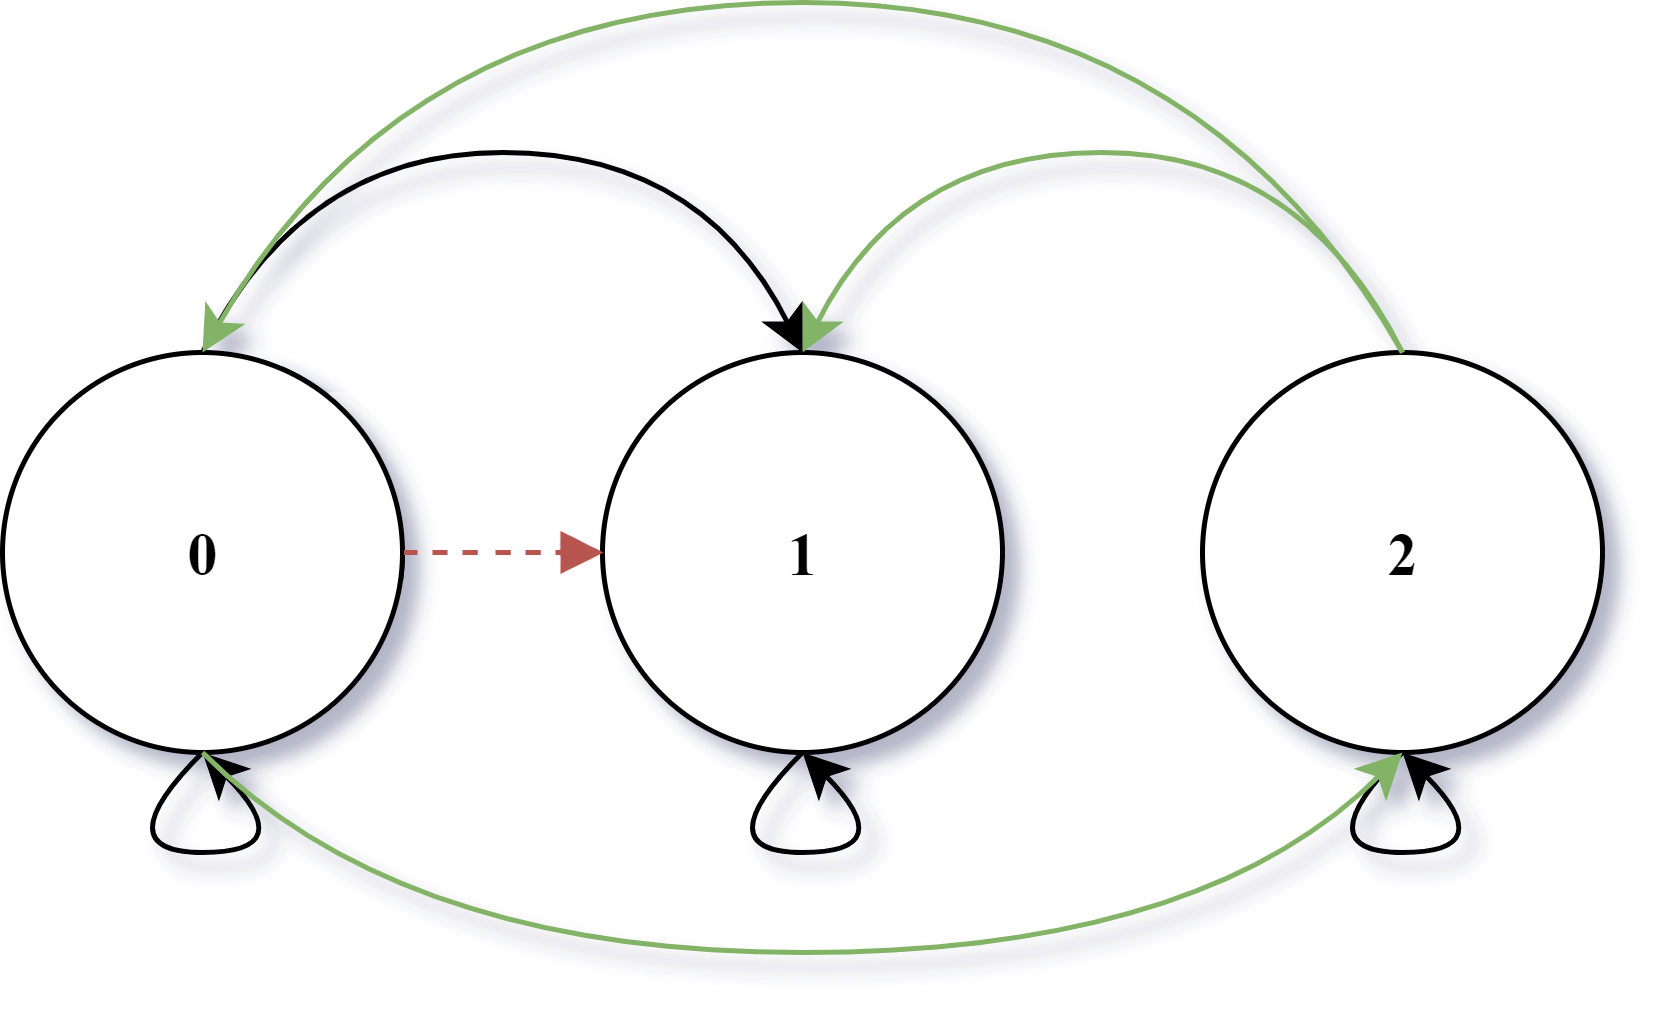
\includegraphics[width=10cm]{diagram.png}
 \caption{Znázornění nepravdivosti výroku tranzitivity grafem. V tomto příkladu byla zvolena \(M=\{0,1,2\}\). Černými šipkami je znázorněna relace $T$, zelenými šipkami je znázorněna relace \(\overline{T}\). Červenou šipkou je znázorněn vztah, který chybí v relaci \(\overline{T}\), aby byla tranzitivní.}
\end{figure}

\section*{Příklad 5}
Je dána množina obsahující deset přirozených čísel mezi 1 a 99, včetně. Dokažte, že existují dvě disjunktní neprázdné podmnožiny této množiny se stejným součtem svých prvků.

\pageline

Protože je daná množina $M$ desetiprvková, existuje $|P(M)| = 2^{10}-1 = 1023$ neprázdných podmnožin, a tedy možných součtů, které mohou vzniknout jako součet prvků libovolné podmnožiny množiny $M$.

Protože je čísel 99, nejvyšší součet, který může vzniknout, je $99+98+\cdots+90=945$. Je zřejmé, že počet existujících neprázdných podmnožin je vyšší než počet součtů, které mohou vzniknout sečtením jednoho až deseti přirozených čísel mezi 1 a 99. Podle Dirichletova principu tak aspoň dvě tyto podmnožiny budou náležet jednomu součtu, čili budou existovat dvě neprázdné podmnožiny se stejným součtem svých prvků. Pokud by takto nalezené podmnožiny nebyly disjunktní, můžeme vytvořit jejich podmnožiny, které nebudou obsahovat jejich průnik. Tyto nové podmnožiny budou disjunktními podmnožinami původní množiny a jejich součet bude stále stejný.
\end{document}